\documentclass[conference]{IEEEtran}
\IEEEoverridecommandlockouts
\usepackage{amsmath,amssymb}
\usepackage{graphicx}
\usepackage{booktabs}
\usepackage{multirow}
\usepackage[hidelinks]{hyperref}

\begin{document}

\title{Risk-Aware Active Perception for Crowd Navigation with a Pan Camera:\\
From Replayed Crowds to Photorealistic RGB-D Simulation}

% TODO: authors and affiliations
\author{\IEEEauthorblockN{Author One, Author Two, Author Three}
\IEEEauthorblockA{Affiliation\\ email@domain}}

\maketitle

\begin{abstract}
A robot with a narrow-field-of-view camera cannot track every pedestrian around it, so it must decide where to look while it moves. We add a risk-aware perception objective to a chance-constrained model predictive controller: the camera is pointed to shrink the uncertainty of the collision constraints that matter for the planned path, including pedestrians not yet detected by a Poisson multi-Bernoulli tracker. In a pre-registered study on 1,800 paired episodes of replayed ETH/UCY crowds, risk-aware gaze beats a fixed camera, look-at-nearest, a time-to-contact heuristic and scanning ($p_\text{Holm}\le0.003$). It performs on par with information-gain gaze and with a decoupled variant that optimizes the same objective after planning the motion, so the benefit comes from the objective rather than joint optimization. With rendered RGB-D images, a person detector and data association in SocNavBench (300 paired runs), success rises from 57\% to 66\% over a fixed camera (95\% CI $[+1, +17]$ points), just missing significance after correction ($p_\text{Holm}=0.056$).
\end{abstract}

\section{Introduction}
Crowd navigation planners usually assume that all nearby pedestrians are observed. A robot with an onboard camera sees only a cone in front of it: people approaching from the side are detected late, and tracks of people who leave the view become stale. Active perception, choosing where to look, is classically driven by information gain~\cite{bajcsy1988}, which reduces uncertainty regardless of whether it matters for the task. We ask whether gaze driven by the \emph{collision risk of the planned motion} navigates crowds more safely.

\section{Method}
\textbf{Planner.} We extend SupeR-MPC~\cite{supermpc}, a robust MPC with chance constraints that accounts for state-estimation, parametric and process uncertainty. The state is the unicycle pose plus a camera pan angle $\phi$, and the inputs are $(v,\omega,\omega_\phi)$. The horizon is $N{=}8$ steps of 0.4\,s.

\textbf{Tracking and prediction.} A Poisson multi-Bernoulli (PMB) tracker~\cite{williams2015} keeps Bernoulli tracks with existence probability $r_j$, plus a Poisson intensity of undetected pedestrians. The intensity is advected by flow channels learned from the scene, and tracks whose position standard deviation exceeds 1\,m are pruned. A Social LSTM~\cite{alahi2016}, trained leave-one-scene-out with rotation augmentation, predicts Gaussian trajectories; the propagated track covariance is added to the network's.

\begin{figure*}[t]
\centering
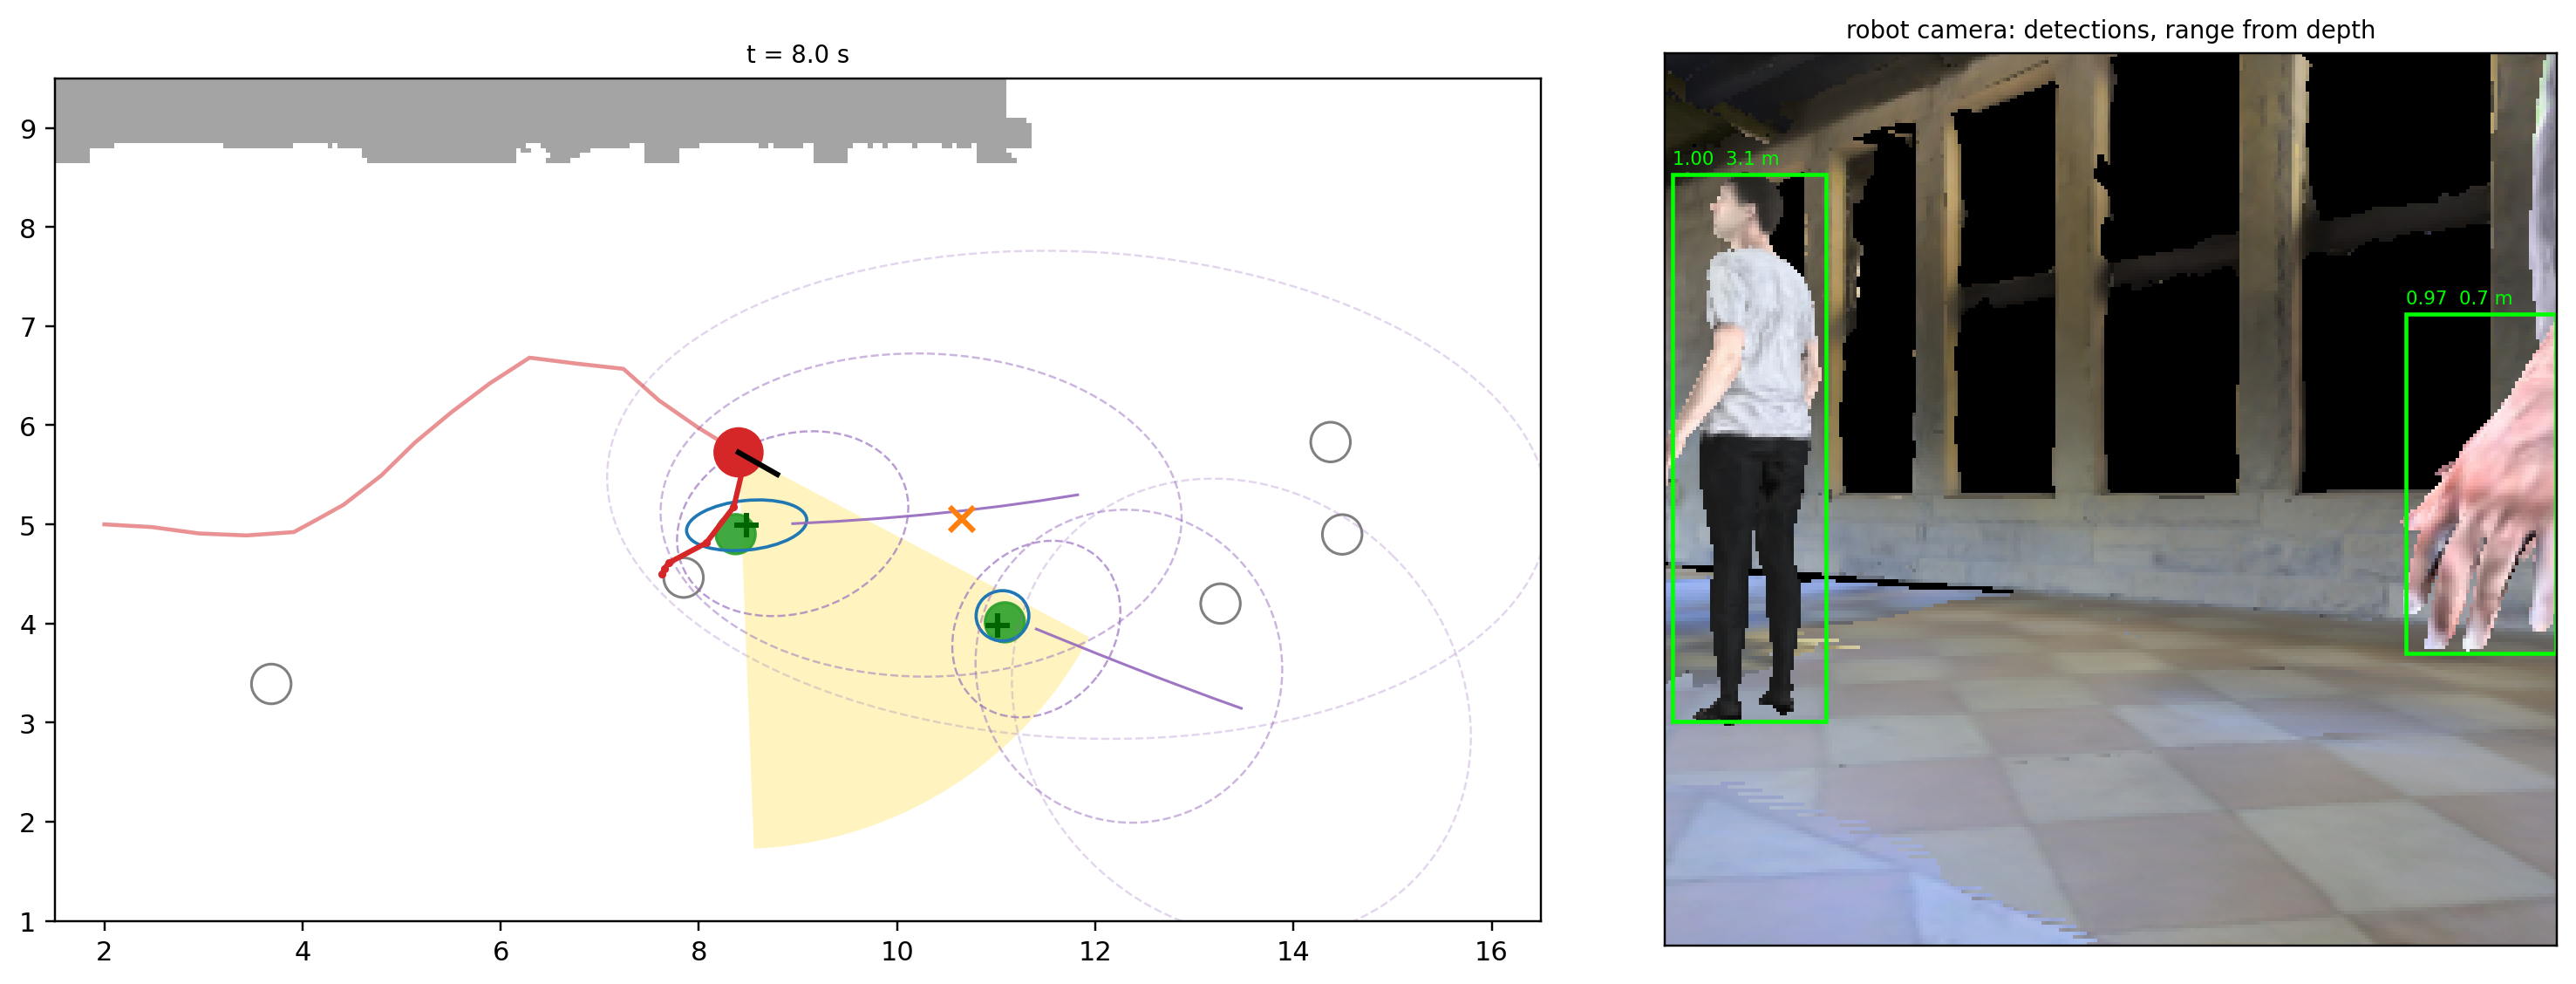
\includegraphics[width=0.64\textwidth]{fig_socnav.png}
\vspace{-2mm}
\caption{Illustrative SocNavBench Zara episode with RGB-D perception. Left: true pedestrians (green: detected), PMB tracks (blue), predictions (purple), the camera cone and the robot's plan. Right: the rendered robot view with detections (score, depth range).}
\label{fig:socnav}
\vspace{-4mm}
\end{figure*}

\textbf{Chance constraints.} For tracked pedestrian $j$ at step $k$,
\begin{equation}
a_{jk}^\top(c_{r,k}-\mu_{jk}) - r_\text{c} \ge \kappa_j \sqrt{2\,a_{jk}^\top(\Sigma_{r,k}+\Sigma_{jk})\,a_{jk}},
\end{equation}
with $\kappa_j=\operatorname{erf}^{-1}(1-2\min(\delta/r_j,\tfrac12))$, so unlikely tracks are constrained less. Undetected pedestrians get one chance constraint per step on the forecast undetected mass inside the robot's collision disk. Constraints always use current information, so safety never relies on views that have not been taken yet.

\textbf{Risk-aware gaze.} The cost rewards views that will shrink future constraint back-offs. Let $\mathrm{vis}_{jk}$ be a smooth visibility model and $\pi_{jm}$ the probability that pedestrian $j$ is first seen at step $m$. The expected covariance is then
\begin{equation}
\begin{aligned}
\tilde\Sigma_{jk} = \Sigma^\text{model}_{jk} &+ \textstyle\prod_{m\le k}(1-\mathrm{vis}_{jm})\,\Sigma^\text{state}_{jk}\\
&+ \textstyle\sum_{m\le k}\pi_{jm} J_{k-m}P_\infty J_{k-m}^\top,
\end{aligned}
\end{equation}
and the cost adds $w\,\rho_{jk}\operatorname{erf}^{-1}(1-2\delta)\sqrt{2a_{jk}^\top(\Sigma_{r,k}+\tilde\Sigma_{jk})a_{jk}}$ for the most collision-relevant pedestrians ($\rho_{jk}$: relevance to the warm-start plan). A second term penalizes the undetected mass left in the path's collision disks after the planned views.

\section{Experiments}
\textbf{Protocol.} Hypotheses, metric, tests and fresh seeds were fixed in a plan committed to version control before running. Success means reaching the goal (0.3\,m) in time without colliding, excluding collisions with pedestrians whose recorded track starts next to the robot (replay starting within 3\,m in 2D; appeared $<2$\,s earlier in SocNavBench), which no gaze policy can prevent. All methods share the planner, tracker and predictor and differ only in gaze: fixed forward camera; scanning; look-at-nearest; a time-to-contact (TTC) heuristic that looks at the most collision-relevant track; information gain ($\log\det$ of expected track covariances); and \emph{decoupled}, which plans the motion first and then optimizes only the camera with our objective. Tests are exact McNemar with Holm correction (one-sided; two-sided vs.\ information gain).

\begin{table}[t]
\centering
\caption{Replayed crowds: 1,800 paired episodes. $p_\text{Holm}$ vs.\ ours.}
\label{tab:replay}
\footnotesize
\begin{tabular}{lccc}
\toprule
Gaze & Success & Never-seen coll. & $p_\text{Holm}$ \\
\midrule
Risk-aware (ours)  & \textbf{0.643} & 964  & -- \\
Decoupled          & 0.644 & 880  & 0.55 \\
Information gain   & 0.629 & 1011 & 0.54 \\
Fixed              & 0.601 & 1605 & 0.003 \\
Look at nearest    & 0.599 & 1811 & 0.002 \\
TTC heuristic      & 0.584 & 1908 & $<$0.001 \\
Scan               & 0.577 & 1603 & $<$0.001 \\
\midrule
Gaze oracle        & 0.686 & 523  & \\
360$^\circ$ camera & 0.858 & 39   & \\
\bottomrule
\end{tabular}
\vspace{-3mm}
\end{table}

\textbf{Replayed crowds.} The robot crosses ETH/UCY scenes (60$^\circ$ FOV, 4\,m range) among replayed, non-reactive pedestrians. The camera model includes occlusion, a 0.9 detection probability and range-dependent noise. The PMB prior is fitted on the first half of each recording, and episodes are drawn from the second half (450 per scene). Risk-aware gaze beats all passive and heuristic gaze strategies (Table~\ref{tab:replay}), with 40\% fewer collisions with never-seen pedestrians than the fixed camera; it does pay with more collisions with tracked pedestrians (757 vs.\ 534). It ties information gain and the decoupled variant. In the ablations (Holm over eight), replacing the PMB tracker by a Kalman filter (0.588, $p_\text{Holm}{=}0.001$) and dropping the tracked-pedestrian gaze term (0.608, $p_\text{Holm}{=}0.03$) significantly lower success; the unseen-pedestrian term is borderline (0.611, $p_\text{Holm}{=}0.07$).

\textbf{Photorealistic RGB-D simulation.} We connected the planner to SocNavBench~\cite{socnavbench}. It replays the same recordings in S3DIS building scans~\cite{armeni2016}, with pedestrians rendered as SURREAL bodies~\cite{varol2017}. Each step, the robot renders a $256{\times}256$ RGB-D image from its pose and pan angle (Fig.~\ref{fig:socnav}). A COCO-trained Faster R-CNN~\cite{ren2015} detects persons, the range comes from the depth pixels inside each box, and detections are associated with the tracks by gated Hungarian matching. On rendered frames, detection precision is 0.93 and recall is 0.88--0.96 within 4\,m, with a median position error of 0.12\,m. Walls enter the MPC as half-plane constraints at the nearest map points. We compare our method with the three best alternatives of the replay study on SocNavBench's 30 curated single-recording episodes with ten fresh seeds each (300 paired runs). Since seeds share episodes, the primary test is a permutation test on the 30 per-episode mean differences.

\begin{table}[t]
\centering
\caption{SocNavBench with RGB-D vision: 300 paired runs; difference with 95\% CI.}
\label{tab:socnav}
\footnotesize
\begin{tabular}{lccc}
\toprule
Gaze & Success & Ours $-$ other (pts) & $p_\text{Holm}$ \\
\midrule
Risk-aware (ours) & \textbf{0.657} & -- & -- \\
Decoupled         & 0.633 & $+2.3$ $[-6.0, +10.3]$ & 0.29 \\
Information gain  & 0.603 & $+5.3$ $[-1.3, +12.3]$ & 0.17 \\
Fixed             & 0.567 & $+9.0$ $[+1.3, +16.7]$ & 0.056 \\
\bottomrule
\end{tabular}
\vspace{-3mm}
\end{table}

With real vision, risk-aware gaze raises success over the fixed camera by 9 points; the confidence interval excludes zero and the uncorrected test is significant ($p{=}0.019$), but after correction it narrowly misses ($p_\text{Holm}{=}0.056$, Table~\ref{tab:socnav}).

\section{Conclusion}
A risk-aware perception objective, which points the camera where uncertainty threatens the planned motion, reliably beats passive and heuristic gaze in replayed crowds, and shows a gain of the same size, just short of corrected significance, with real RGB-D perception in a photorealistic simulator. Optimizing gaze jointly with the motion brought no measurable benefit over a decoupled two-stage version of the same objective, and information-gain gaze performed comparably. Limitations, and next steps, are non-reactive replayed pedestrians, ground-truth localization and the short detection range.

\begin{thebibliography}{10}
\footnotesize
\bibitem{bajcsy1988} R.~Bajcsy, ``Active perception,'' \emph{Proc.\ IEEE}, vol.~76, no.~8, pp.~966--1005, 1988.
% TODO: complete the SupeR-MPC reference
\bibitem{supermpc} Zhu, Simeon, and Cognetti, ``SupeR-MPC,'' \emph{IEEE Robot.\ Autom.\ Lett.}, 2025.
\bibitem{williams2015} J.~L.~Williams, ``Marginal multi-Bernoulli filters: RFS derivation of MHT, JIPDA, and association-based MeMBer,'' \emph{IEEE Trans.\ Aerosp.\ Electron.\ Syst.}, vol.~51, no.~3, pp.~1664--1687, 2015.
\bibitem{alahi2016} A.~Alahi \emph{et al.}, ``Social LSTM: Human trajectory prediction in crowded spaces,'' in \emph{Proc.\ CVPR}, 2016.
\bibitem{socnavbench} A.~Biswas \emph{et al.}, ``SocNavBench: A grounded simulation testing framework for evaluating social navigation,'' \emph{ACM Trans.\ Human-Robot Interact.}, vol.~11, no.~3, 2022.
\bibitem{armeni2016} I.~Armeni \emph{et al.}, ``3D semantic parsing of large-scale indoor spaces,'' in \emph{Proc.\ CVPR}, 2016.
\bibitem{varol2017} G.~Varol \emph{et al.}, ``Learning from synthetic humans,'' in \emph{Proc.\ CVPR}, 2017.
\bibitem{ren2015} S.~Ren \emph{et al.}, ``Faster R-CNN: Towards real-time object detection with region proposal networks,'' in \emph{Proc.\ NeurIPS}, 2015.
\end{thebibliography}

\end{document}
